%%%%%%%%%%%%%%%%%%%%%%%%%%%%%%%%%%%%%%%%%
% Jacobs Landscape Poster
% LaTeX Template
%
% Original poster by:
% Computational Physics and Biophysics Group, Jacobs University
% https://teamwork.jacobs-university.de:8443/confluence/display/CoPandBiG/LaTeX+Poster
% 
% Also modified by:
% Nathaniel Johnston (nathaniel@njohnston.ca)
% Sarah Scheffler (sscheff@bu.edu, 4/26/17)
%
% This template has been downloaded from:
% http://www.LaTeXTemplates.com
%
% License:
% CC BY-NC-SA 3.0 (http://creativecommons.org/licenses/by-nc-sa/3.0/)
%
%%%%%%%%%%%%%%%%%%%%%%%%%%%%%%%%%%%%%%%%%

%----------------------------------------------------------------------------------------
%	PACKAGES AND OTHER DOCUMENT CONFIGURATIONS
%----------------------------------------------------------------------------------------

\documentclass[final]{beamer}

\usepackage[scale=1.00]{beamerposter} % Use the beamerposter package for laying out the poster

\usetheme{confposter} % Use the confposter theme supplied with this template


\setbeamercolor{block title}{fg=bured,bg=white} % Colors of the block titles
\setbeamercolor{block body}{fg=black,bg=white} % Colors of the body of blocks
\setbeamercolor{block alerted title}{fg=white,bg=bured!70} % Colors of the highlighted block titles
\setbeamercolor{block alerted body}{fg=black,bg=bured!10} % Colors of the body of highlighted blocks
% Many more colors are available for use in beamerthemeconfposter.sty

%-----------------------------------------------------------
% Define the column widths and overall poster size
% To set effective sepwid, onecolwid and twocolwid values, first choose how many columns you want and how much separation you want between columns
% In this template, the separation width chosen is 0.024 of the paper width and a 4-column layout
% onecolwid should therefore be (1-(# of columns+1)*sepwid)/# of columns e.g. (1-(4+1)*0.024)/4 = 0.22
% Set twocolwid to be (2*onecolwid)+sepwid = 0.464
% Set threecolwid to be (3*onecolwid)+2*sepwid = 0.708
\usepackage{fontspec}
\newlength{\sepwid}
\newlength{\onecolwid}
\newlength{\twocolwid}
\newlength{\threecolwid}
\setlength{\paperwidth}{40in} % A0 width: 46.8in
\setlength{\paperheight}{30in} % A0 height: 33.1in
\setlength{\sepwid}{0.024\paperwidth} % Separation width (white space) between columns
\setlength{\onecolwid}{0.22\paperwidth} % Width of one column
\setlength{\twocolwid}{0.464\paperwidth} % Width of two columns
\setlength{\threecolwid}{0.708\paperwidth} % Width of three columns
\setlength{\topmargin}{-0.5in} % Reduce the top margin size
%-----------------------------------------------------------
%\setmainfont{Noto Sans}
\usepackage{graphicx}  % Required for including images
\usepackage{booktabs} % Top and bottom rules for tables
\usepackage{biblatex}
\addbibresource{2539190.bib}
%----------------------------------------------------------------------------------------
%	TITLE SECTION 
%----------------------------------------------------------------------------------------

\title{Eftychis: Sentiment Analysis on Twitter Users} % Poster title

\author{Anton M. Paquin, William J. Chen} % Author(s) %TODO: ordering?

\institute{\{paquin,chenwill\}@bu.edu} % Institution(s) or emails

%----------------------------------------------------------------------------------------

\begin{document}

\addtobeamertemplate{block end}{}{\vspace*{2ex}} % White space under blocks
\addtobeamertemplate{block alerted end}{}{\vspace*{2ex}} % White space under highlighted (alert) blocks

\setlength{\belowcaptionskip}{2ex} % White space under figures
\setlength\belowdisplayshortskip{2ex} % White space under equations

\begin{frame}[t] % The whole poster is enclosed in one beamer frame

\begin{columns}[t] % The whole poster consists of three major columns, the second of which is split into two columns twice - the [t] option aligns each column's content to the top

\begin{column}{\sepwid}\end{column} % Empty spacer column

\begin{column}{\onecolwid} % The first column


%----------------------------------------------------------------------------------------
%	SECTION 
%----------------------------------------------------------------------------------------

\begin{block}{\textbf{Powered by:}}
\begin{center}
\includegraphics[
width=0.7\linewidth]{Elasticsearch-Logo-Color-V-sm.png} \end{center}

%
\includegraphics[width=0.5\linewidth]{Kibana-Logo-Color-H} 


\end{block}

%----------------------------------------------------------------------------------------
%	SECTION 
%----------------------------------------------------------------------------------------

\begin{block}{Data Acquisition}

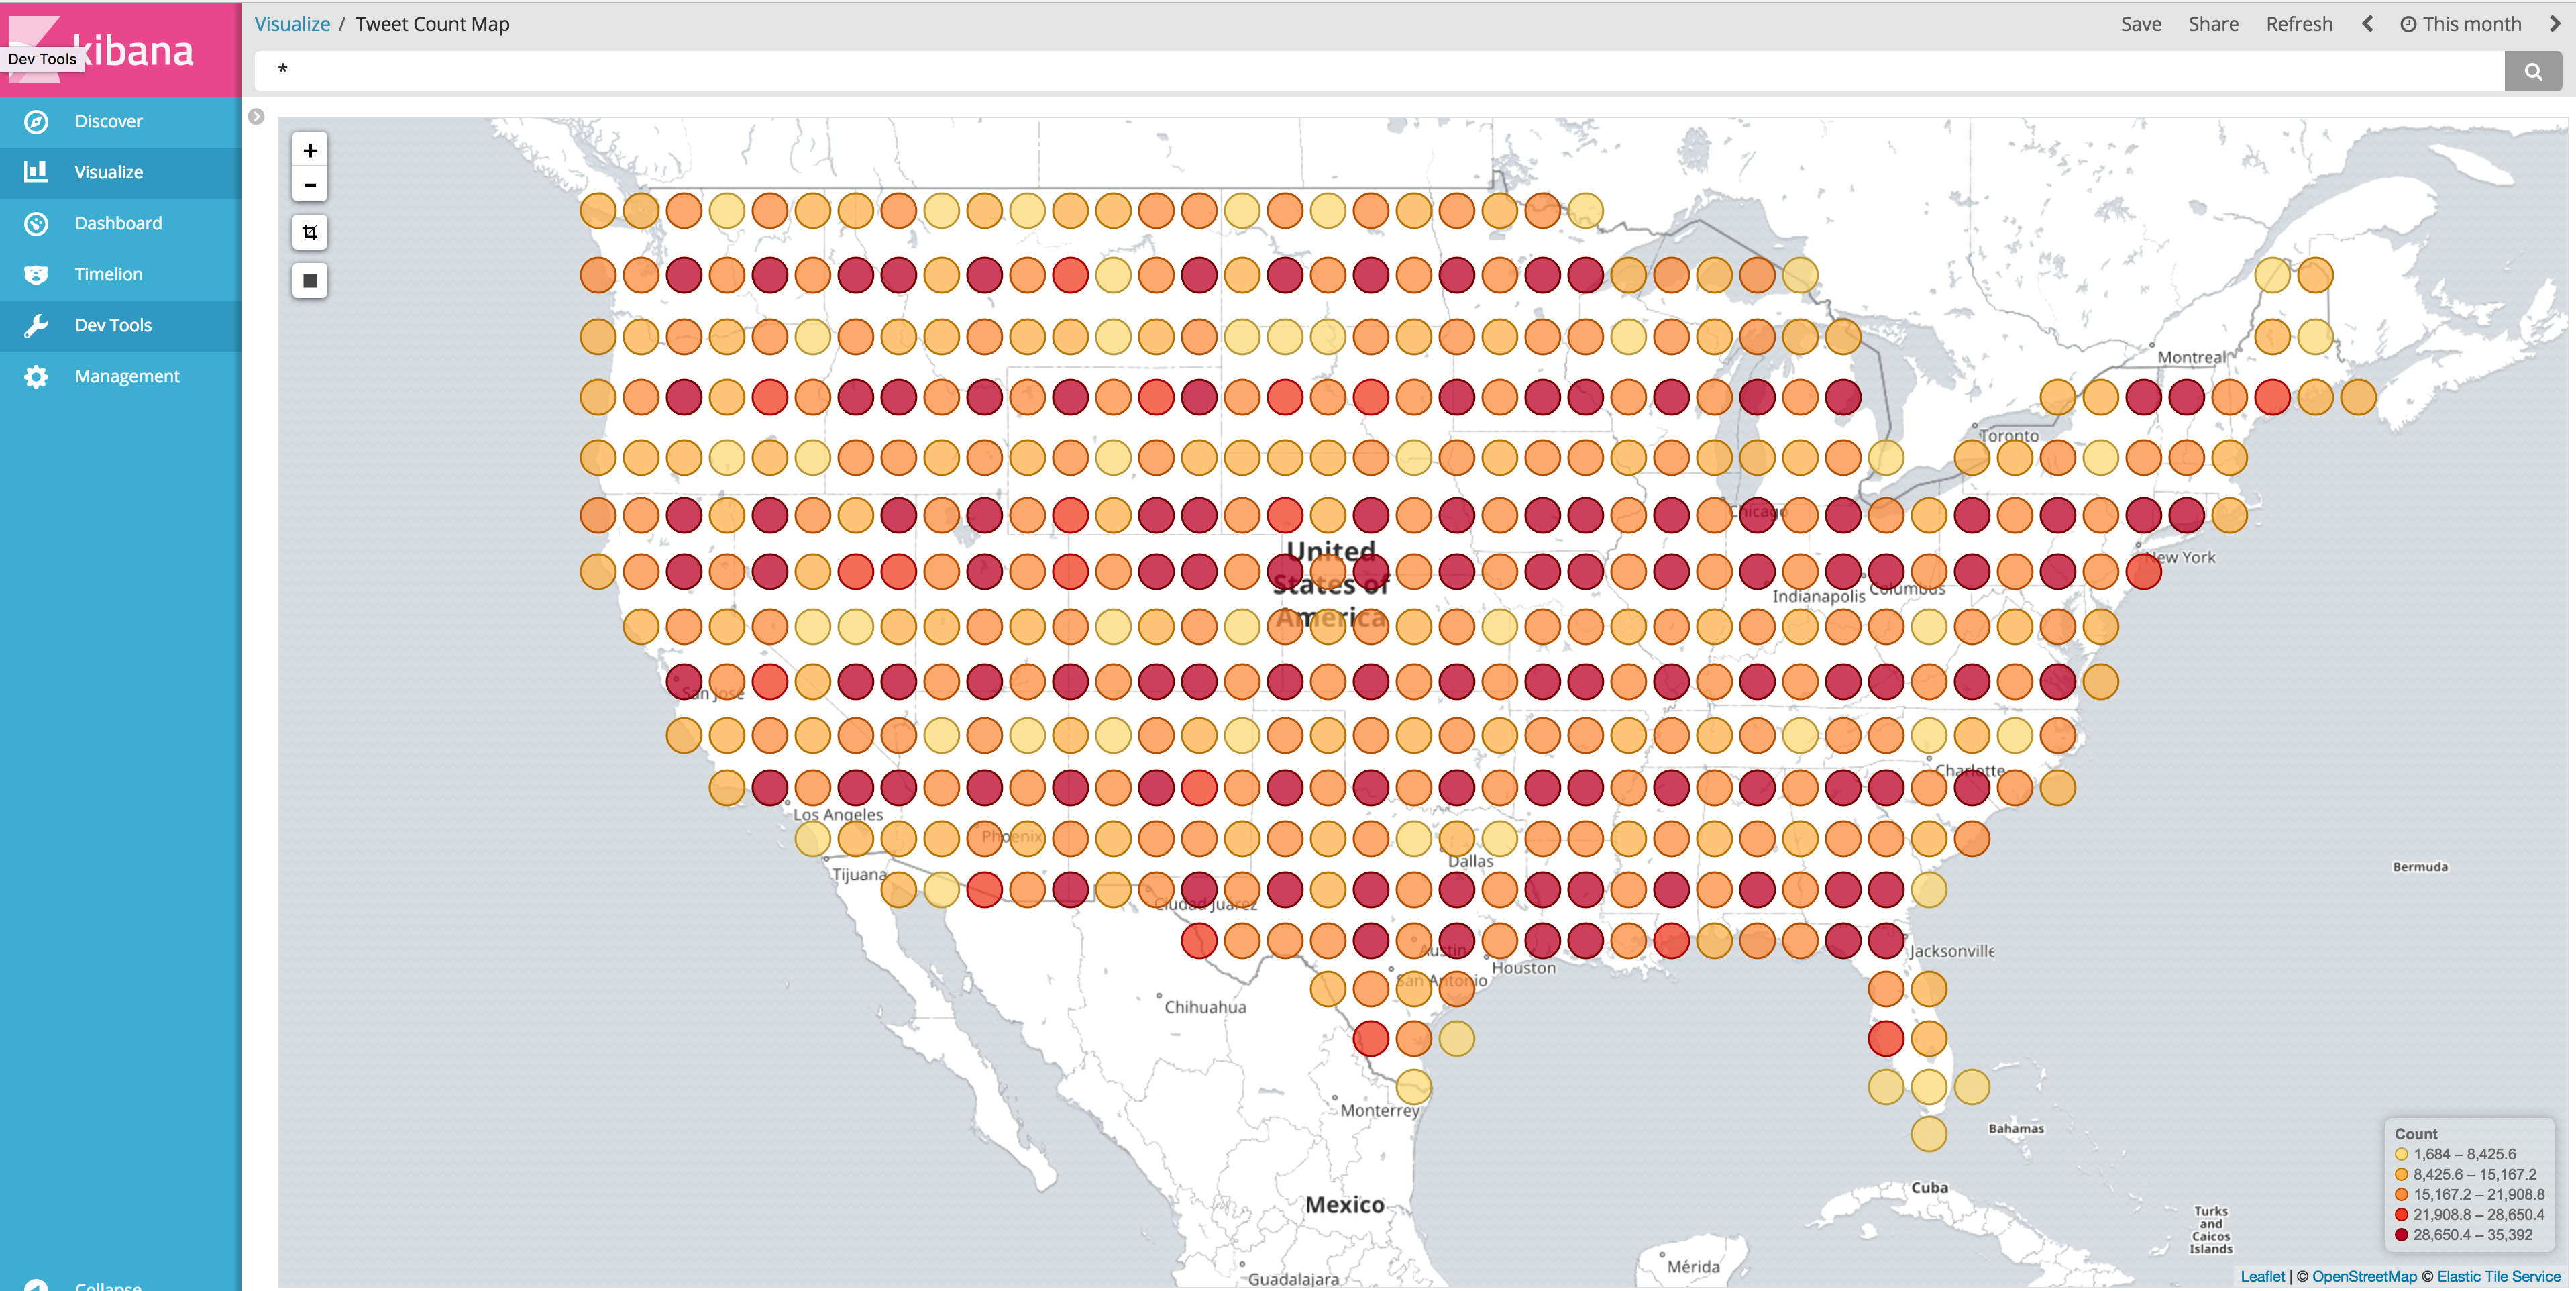
\includegraphics[width=1\linewidth]{screenshot.png} 
\newline


Using a Google Cloud Platform virtual server and the Twitter API, we were able to scrape \textbf{23,585,039} tweets over the span of \textbf{10 days} from the Twitter social network. To obtain a geographically diverse set of tweets, we first list of \textbf{1054 coordinate pairs} that were equally spaced (\textbf{65km} apart) across the continental United States in a grid. We then made hourly API calls that requested 100 tweets located within 65km of each coordinate pair. \newline


The collected data was then ingested into the Elasticsearch engine, which performed word tokenization and snowball filtering (word stemming). \newline

Elasticsearch also allowed us to identify the top most commonly observed words amongst all of the tweets we obtained. While the top three words were "https", "t.co", and "rt", indicating URLs and retweets, many of the other words were pronouns such as "you", "me", etc

\end{block}

%----------------------------------------------------------------------------------------

\end{column} % End of the first column

\begin{column}{\sepwid}\end{column} % Empty spacer column

\begin{column}{\twocolwid} % Begin a column which is two columns wide (column 2)

%----------------------------------------------------------------------------------------
%	SECTION 
%----------------------------------------------------------------------------------------

\begin{block}{Data Analysis}
% This is just here for the title
\end{block} 

\begin{columns}[t,totalwidth=\twocolwid] % Split up the two columns wide column

\begin{column}{\onecolwid}\vspace{-.6in} % The first column within column 2 (column 2.1)

%----------------------------------------------------------------------------------------
%	SECTION 
%----------------------------------------------------------------------------------------

\begin{block}{Label Propagation}

To begin our sentiment analysis, we constructed an undirected graph with nodes representing each of the top 2000 words. Edges were created between each node with an edge weight indicating the frequency of tweets containing words A and B divided by the sum of tweets containing A and every other node. The result is a 2000-by-2000 matrix indicating probability that word i and j are related. Mathematically speaking, 
we calculate 
\begin{equation}
T_{i,j} = \frac{w_{i,j}}{\sum_{k=0, i!=k}^{2000} w_{i,k}}
\end{equation}
for all nodes i,j. 

From the 2000 most popular words, we created a list of "clamp words" containing positive words, and another for negative words.  We initialize a 2000-by-2 matrix y with each element set to (0,0), set positive clamps to (1,0), and set negative clamps to (0,1). Using y, T, and a constant $\alpha$ (= 0.3), we produce a 2000-by-2 matrix y' that relates non-clamp words with their clamped words via the equation:

\begin{equation}
\textbf{y'} = \alpha \textbf{Ty} + (1-\alpha)\textbf{y}
\end{equation}

With the y' matrix, we are able to compute a "raw happiness score" for all of the scraped tweets.

\end{block}


%----------------------------------------------------------------------------------------
%	SECTION 
%----------------------------------------------------------------------------------------

%----------------------------------------------------------------------------------------

\end{column} % End of column 2.1

\begin{column}{\onecolwid}\vspace{-.6in} % The second column within column 2 (column 2.2)

%----------------------------------------------------------------------------------------
%	OVERVIEW
%----------------------------------------------------------------------------------------

\begin{block}{Clustering Analysis/Regression?}


\end{block}

%----------------------------------------------------------------------------------------
%	GLOSSARY
%----------------------------------------------------------------------------------------

\begin{alertblock}{Glossary}
\textbf{Clamp} - Ground truth
\end{alertblock}


%----------------------------------------------------------------------------------------

\end{column} % End of column 2.2

\end{columns} % End of the split of column 2 - any content after this will now take up 2 columns width



%----------------------------------------------------------------------------------------

\begin{columns}[t,totalwidth=\twocolwid] % Split up the two columns wide column again

\begin{column}{\onecolwid} % The first column within column 2 (column 2.1)


%----------------------------------------------------------------------------------------

\end{column} % End of column 2.1

\begin{column}{\onecolwid} % The second column within column 2 (column 2.2)



%----------------------------------------------------------------------------------------

\end{column} % End of column 2.2

\end{columns} % End of the split of column 2

\end{column} % End of the second column

\begin{column}{\sepwid}\end{column} % Empty spacer column

\begin{column}{\onecolwid} % The third column

%----------------------------------------------------------------------------------------
%	DNS CACHE POISONING THROUGH EMAIL
%----------------------------------------------------------------------------------------

\begin{block}{Conclusion}


\end{block}



%----------------------------------------------------------------------------------------
%	REFERENCES
%----------------------------------------------------------------------------------------

\begin{block}{References}

%{Yen-Jen Tai and Hung-Yu Kao. 2013. Automatic Domain-Specific Sentiment Lexicon Generation with Label Propagation. In Proceedings of International Conference on Information Integration and %Web-based Applications & Services (IIWAS '13). ACM, New York, NY, USA, , Pages 53 , 10 pages. DOI: http://dx.doi.org/10.1145/2539150.2539190}

\nocite{*} % Insert publications even if they are not cited in the poster
%\small{\bibliographystyle{plain}
%\bibliography{2539190.bib}\vspace{0.75in}
\printbibliography
\end{block}

%----------------------------------------------------------------------------------------
%	ACKNOWLEDGEMENTS
%----------------------------------------------------------------------------------------

\setbeamercolor{block title}{fg=red,bg=white} % Change the block title color

\begin{block}{Acknowledgements}

We would like to extend a warm thanks to Professor Evimaria Terzi for her lectures on data analysis techniques used in this project as part of CS506 - Computational Tools for Data Science.
In addition, we 
\newline

\end{block}





%----------------------------------------------------------------------------------------

\end{column} % End of the third column
\begin{column}{\sepwid}\end{column} % Empty spacer column

\end{columns} % End of all the columns in the poster

%----------------------------------------------------------------------------------------
%	LOGO - this will likely need some manual readjustment
%----------------------------------------------------------------------------------------
\vspace*{\fill}
\begin{tikzpicture}{}[remember picture,overlay]
\begin{scope}[transform canvas={xshift=-3cm, yshift=-3.5cm}]
\node[anchor=south east] at (current page.south east) {\null\hfill
\includegraphics[width=.05\linewidth]{bucompsci} \textsf{\large{~@BUCompSci}}};
\end{scope}
\end{tikzpicture}

\end{frame} % End of the enclosing frame

\end{document}
